
\documentclass[border=12pt]{standalone}
\usepackage{pgfplots}
\pgfplotsset{compat=1.18}
\begin{document}
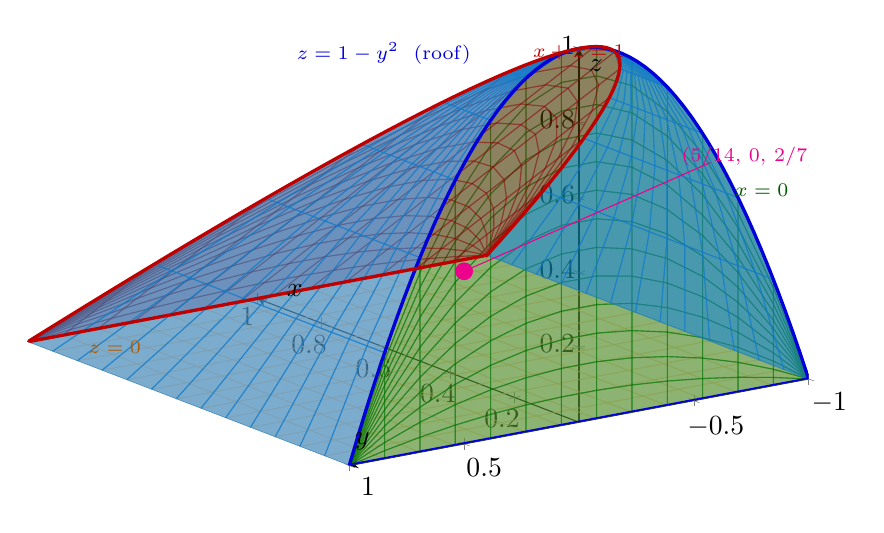
\begin{tikzpicture}
\begin{axis}[
    width=11.5cm, height=9.0cm,
    view={-125}{22}, xlabel={$x$}, ylabel={$y$}, zlabel={$z$},
    xmin=0, xmax=1, ymin=-1, ymax=1, zmin=0, zmax=1,
    axis lines=center, grid=major, grid style={gray!20},
    samples=14, samples y=14,
    every node/.style={execute at begin node=\setlength{\baselineskip}{1.1em}}]

  % base z = 0
  \addplot3[surf, orange!45, opacity=.40, shader=flat, domain=0:1, y domain=-1:1] (x, y, 0);
  % end cap x = 0
  \addplot3[surf, green!45!black, opacity=.45, shader=flat, domain=-1:1, y domain=0:1]
     ({0.0001*x}, x, {y*(1-x*x)});
  % slanted plane x + z = 1
  \addplot3[surf, red!55!black, opacity=.32, shader=flat, domain=-1:1, y domain=0:1]
     ({1-y*(1-x*x)}, x, {y*(1-x*x)});
  % roof z = 1 - y^2
  \addplot3[surf, cyan!60!blue, opacity=.55, shader=flat, domain=-1:1, y domain=0:1]
     ({y*x*x}, x, 1-x*x);

  % key edges
  \addplot3[very thick, blue!85!black, domain=-1:1, samples=60] ({0.0001*x}, x, 1-x*x);
  \addplot3[very thick, red!75!black, domain=-1:1, samples=60] ({x*x}, x, 1-x*x);

  % center of mass
  \addplot3[only marks, mark=*, mark size=3pt, magenta] coordinates {(0.3571,0,0.2857)};

  \node[blue!85!black, font=\scriptsize] at (axis cs:0.05,0.78,1.06) {$z=1-y^2$\ \ (roof)};
  \node[red!75!black, font=\scriptsize] at (axis cs:0.75,-1.05,0.62) {$x+z=1$};
  \node[green!35!black, font=\scriptsize] at (axis cs:0.06,-0.88,0.50) {$x=0$};
  \node[orange!70!black, font=\scriptsize] at (axis cs:0.80,0.90,0.04) {$z=0$};
  \node[magenta, font=\scriptsize] at (axis cs:0.15,-0.95,0.55) {$(5/14,\,0,\,2/7)$};
  \draw[->, magenta, thin] (axis cs:0.22,-0.88,0.52) -- (axis cs:0.3571,0,0.2857);
\end{axis}
\end{tikzpicture}
\end{document}
